\chapter{MODIS y VIIRS frente a frente}\label{cap:modisviirs}

\objetivos{
\begin{itemize}
  \item Describir cada instrumento: plataformas, bandas usadas para el fuego y resolución.
  \item Explicar qué es la saturación de un detector y cómo afecta a cada sensor.
  \item Enumerar todas las diferencias entre MODIS y VIIRS que influyen en el número de focos.
  \item Leer una imagen real en la que ambos sensores observan la misma región el mismo día.
\end{itemize}}

\section{Dos generaciones}

Los capítulos anteriores han ido presentando piezas sueltas de los dos instrumentos. Este las
reúne. Leerlo con atención vale la pena: la lista de diferencias de la
sección~\ref{sec:diferencias} es, en la práctica, la lista de cosas que la armonización tiene
que corregir.

\section{MODIS}

MODIS es un radiómetro de 36 bandas espectrales, desde el visible hasta el infrarrojo térmico,
diseñado en los años noventa como instrumento de propósito general del Sistema de Observación de
la Tierra de la NASA. Se construyeron dos unidades casi idénticas:

\begin{itemize}
  \item \textbf{Terra}, lanzado en diciembre de 1999, en órbita de mañana (10:30);
  \item \textbf{Aqua}, lanzado en mayo de 2002, en órbita de tarde (13:30).
\end{itemize}

Las 36 bandas tienen tres resoluciones distintas en el nadir: 250~m (2 bandas), 500~m (5
bandas) y 1~km (29 bandas). Todas las bandas térmicas son de 1~km, y por eso el producto de
fuego tiene esa resolución. Las que usa el algoritmo de fuego son las de la
tabla~\ref{tab:bandas-modis}.

\begin{table}[ht]
\centering
\begin{tabular}{clcl}
\toprule
Banda & Longitud de onda & Saturación & Papel en la detección \\
\midrule
21 & 3,96 \um & $\approx 500$ K & canal de fuego, rango alto \\
22 & 3,96 \um & $\approx 331$ K & canal de fuego, rango bajo y menos ruido \\
31 & 11,0 \um & $\approx 400$ K (Terra) & temperatura del fondo, nubes \\
   &  & $\approx 340$ K (Aqua) & \\
32 & 12,0 \um & & máscara de nubes \\
1, 2 & 0,65 y 0,86 \um & & reflectancia: nubes, agua, brillo solar \\
7 & 2,1 \um & & rechazo de brillo solar y costas \\
\bottomrule
\end{tabular}
\caption{Bandas de MODIS que intervienen en la detección de fuego.}
\label{tab:bandas-modis}
\end{table}

Llama la atención que haya \emph{dos} bandas en la misma longitud de onda. La razón es la
saturación.

\section{Saturación}

Un detector convierte radiancia en una señal eléctrica, y la electrónica solo puede representar
un intervalo limitado de valores. Si la radiancia supera el máximo, el detector entrega su valor
tope y ya no dice cuánto más había.

\begin{definicion}{saturación}
Un detector se satura cuando la radiancia que recibe supera el máximo que puede medir. La
\emph{temperatura de saturación} es la temperatura de brillo correspondiente a ese máximo. Por
encima de ella todas las mediciones valen lo mismo.
\end{definicion}

Hay aquí un compromiso inevitable. Un detector pensado para medir con precisión temperaturas de
la superficie (entre 250 y 330~K) se satura enseguida con un fuego. Uno pensado para no saturarse
con un fuego mide el fondo con poco detalle y más ruido. MODIS lo resuelve con las dos bandas de
4~\um: la \textbf{22} es precisa pero se satura hacia 331~K; la \textbf{21} es ruidosa pero
aguanta hasta unos 500~K. El algoritmo usa la banda 22 siempre que puede y cambia a la 21 cuando
la 22 se satura. En ambos casos el resultado se llama simplemente $T_4$.

\begin{figure}[ht]
\centering
\begin{tikzpicture}
\begin{axis}[width=12.5cm,height=6.4cm,xmin=280,xmax=560,ymin=280,ymax=560,
  xlabel={Temperatura de brillo real del píxel (K)},
  ylabel={Temperatura de brillo medida (K)},
  legend style={at={(0.03,0.96)},anchor=north west,font=\small,draw=ceniza!40},
  grid=major,grid style={ceniza!15}]
\addplot[ceniza,dashed,domain=280:560] {x};
\addplot[modis,very thick] coordinates {(280,280)(331,331)(560,331)};
\addplot[modis!55,very thick,dashdotted] coordinates {(280,280)(500,500)(560,500)};
\addplot[viirs,very thick] coordinates {(280,280)(367,367)(560,367)};
\legend{medición ideal,MODIS banda 22,MODIS banda 21,VIIRS banda I4}
\end{axis}
\end{tikzpicture}
\caption{Respuesta de los canales de 4~\um{} (esquema). Cada detector sigue a la temperatura
real hasta su punto de saturación y a partir de ahí se queda plano.}
\label{fig:saturacion}
\end{figure}

\section{VIIRS}

VIIRS es el instrumento que sucede a MODIS (y al más antiguo AVHRR) dentro del sistema de
satélites meteorológicos polares de Estados Unidos. Vuela en:

\begin{itemize}
  \item \textbf{Suomi NPP}, lanzado en octubre de 2011;
  \item \textbf{NOAA-20}, lanzado en noviembre de 2017;
  \item \textbf{NOAA-21}, lanzado en noviembre de 2022.
\end{itemize}

Los tres comparten la órbita de las 13:30. VIIRS tiene 22 bandas de dos tipos: las bandas
\textbf{I} (de \emph{imagery}), con 375~m de resolución en el nadir, y las bandas \textbf{M}
(de \emph{moderate}), con 750~m. Existen dos productos de fuego, uno por cada resolución; el que
distribuye FIRMS como producto principal, y el que nos ocupa, es el de \textbf{375~m}.

\begin{table}[ht]
\centering
\begin{tabular}{clcl}
\toprule
Banda & Longitud de onda & Saturación & Papel en la detección \\
\midrule
I4 & 3,74 \um & 367 K & canal de fuego \\
I5 & 11,45 \um & $\approx 380$ K & temperatura del fondo, nubes \\
I1, I2, I3 & 0,64; 0,86; 1,61 \um & & nubes, agua, brillo solar \\
M13 & 4,05 \um{} (750 m) & $\approx 634$ K & potencia radiativa del fuego \\
\bottomrule
\end{tabular}
\caption{Bandas de VIIRS que intervienen en el producto de fuego de 375~m.}
\label{tab:bandas-viirs}
\end{table}

Dos detalles de la tabla tendrán consecuencias más adelante. El canal de fuego I4 está en
3,74~\um, no en 3,96: algo más lejos de la absorción del CO$_2$ y algo más sensible a la luz
solar reflejada. Y se satura a 367~K, una temperatura que un fuego mediano alcanza con facilidad
en un píxel tan pequeño. Por eso la \emph{potencia} del fuego no se calcula con I4 sino con la
banda M13, de 750~m, que tiene un rango mucho mayor (capítulo~\ref{cap:frp}).

\section{La comparación completa}\label{sec:diferencias}

\begin{table}[ht]
\centering
\renewcommand{\arraystretch}{1.25}
\begin{tabularx}{\textwidth}{>{\raggedright\arraybackslash}p{4.2cm}>{\raggedright\arraybackslash}X>{\raggedright\arraybackslash}X}
\toprule
 & \textbf{MODIS} & \textbf{VIIRS (375 m)} \\
\midrule
Satélites & Terra, Aqua & Suomi NPP, NOAA-20, NOAA-21 \\
Datos de focos desde & noviembre de 2000 & enero de 2012 \\
Altura de la órbita & 705 km & 824 km \\
Hora de cruce & 10:30 y 13:30 & 13:30 \\
Ancho de la franja & 2330 km (huecos en el ecuador) & 3040 km (sin huecos) \\
Píxel en el nadir & 1 km & 375 m \\
Píxel en el borde & $\approx 2{,}0 \times 4{,}8$ km & $\approx 0{,}8 \times 0{,}8$ km \\
Área del píxel (nadir) & 1 km$^2$ & 0,14 km$^2$ \\
Canal de fuego & 3,96 \um{} (bandas 21 y 22) & 3,74 \um{} (I4) \\
Canal de fondo & 11,0 \um{} (banda 31) & 11,45 \um{} (I5) \\
Saturación a 4 \um & $\approx 500$ K & 367 K \\
Duplicados por pajarita & sí & casi eliminados a bordo \\
Confianza & número de 0 a 100 & baja, nominal, alta \\
Continuidad & consultar plan y deriva orbital & SNPP histórico; NOAA-20/21 para continuidad \\
\bottomrule
\end{tabularx}
\caption{Diferencias entre los dos sensores que influyen en el registro de focos.}
\label{tab:comparacion}
\end{table}

Cada fila de la tabla~\ref{tab:comparacion} empuja el conteo en una dirección. Conviene
repasarlas una a una y preguntarse: \emph{ante los mismos fuegos, ¿esta diferencia hace que
VIIRS cuente más o menos?}

\begin{description}[leftmargin=1.2em,style=nextline]
  \item[Píxel más pequeño: más detecciones de fuegos chicos.] Un fuego ocupa una fracción siete
  veces mayor de un píxel de VIIRS que de uno de MODIS. Fuegos que MODIS no alcanza a
  distinguir del fondo sí superan el umbral en VIIRS. Es el efecto dominante para quemas
  agrícolas pequeñas.
  \item[Píxel más pequeño: más píxeles por fuego grande.] Un frente de fuego de 3~km cruza unos
  tres píxeles de MODIS y unos ocho de VIIRS. Los dos <<ven>> el incendio, pero VIIRS lo cuenta
  casi tres veces más. Este efecto no añade información sobre la actividad; solo cambia la
  unidad.
  \item[Poco crecimiento en los bordes: más detecciones lejos del nadir.] En el borde de la
  franja MODIS pierde casi toda su sensibilidad a fuegos pequeños; VIIRS apenas pierde. La
  ventaja de VIIRS es mayor para lo observado de lado que para lo observado desde arriba.
  \item[Franja más ancha: más días observados.] En latitudes bajas, VIIRS observa cada lugar
  todos los días y MODIS no.
  \item[Más satélites: más pasadas.] Con tres VIIRS en vuelo hay tres oportunidades de
  detección cada tarde.
  \item[Sin Terra: se pierde la mañana.] La serie de MODIS incluye observaciones a las 10:30
  que VIIRS no puede reproducir. Esta es la única diferencia que juega a favor de MODIS.
\end{description}

\begin{intuicion}[Dos tipos de <<más>>]
Es útil separar las diferencias en dos familias. Unas hacen que VIIRS vea fuegos que MODIS
\emph{no ve}: píxel pequeño, bordes, huecos. Otras hacen que VIIRS cuente \emph{más veces} lo
que MODIS también ve: más píxeles por fuego, más satélites. Las segundas se corrigen eligiendo
bien la unidad de conteo. Las primeras no tienen arreglo exacto, porque la información
sencillamente no está en MODIS; solo se pueden compensar en promedio, con estadística.
\end{intuicion}

\section{Cuánto más detecta VIIRS}

No hay una cifra única, y esa es una de las lecciones centrales del libro. Los estudios que
compararon ambos sensores en sus primeros años encontraron que, en la parte central de la franja,
VIIRS de 375~m producía del orden de un cuarto más de detecciones que MODIS, y que fuera de esa
zona central la diferencia subía a alrededor del 70\,{}\%. Para las detecciones nocturnas, donde
el canal I4 trabaja sin la interferencia del Sol, la ventaja es todavía mayor.

Pero esos son promedios globales. La razón entre los conteos depende del tipo de fuego:

\begin{itemize}
  \item donde predominan \textbf{quemas pequeñas y breves} (agricultura, pastos), VIIRS puede
  detectar varias veces más que MODIS, porque casi todo está por debajo del límite de MODIS;
  \item donde predominan \textbf{incendios grandes e intensos} (bosque boreal, sabanas), ambos
  detectan casi todos los eventos y la diferencia se debe sobre todo al número de píxeles por
  fuego.
\end{itemize}

\begin{parareto}
La consecuencia es que \textbf{un solo factor de conversión para todo el planeta es una mala
armonización}. La razón VIIRS/MODIS hay que estimarla para cada región, y probablemente también
para cada época del año, porque el tipo de fuego cambia con la estación. Esto no es una
complicación opcional: es el núcleo técnico del reto y lo que distinguirá una solución cuidadosa
de una ingenua.
\end{parareto}

\section{Un caso real: el centro del Perú, 15 de septiembre de 2024}

La figura~\ref{fig:worldview} muestra dos imágenes reales tomadas el mismo día sobre la misma
zona: aproximadamente entre 9$^\circ$ y 14$^\circ$ de latitud sur y entre 72,5$^\circ$ y
77,5$^\circ$ de longitud oeste. El recuadro abarca la costa central, la sierra de Junín, Pasco y
Huancavelica y la selva central. Los puntos rojos son las detecciones de fuego de cada sensor.

\begin{figure}[ht]
\centering
\begin{subfigure}[t]{0.485\textwidth}
  \begin{tikzpicture}
    \node[inner sep=0,anchor=south west] (img) at (0,0) {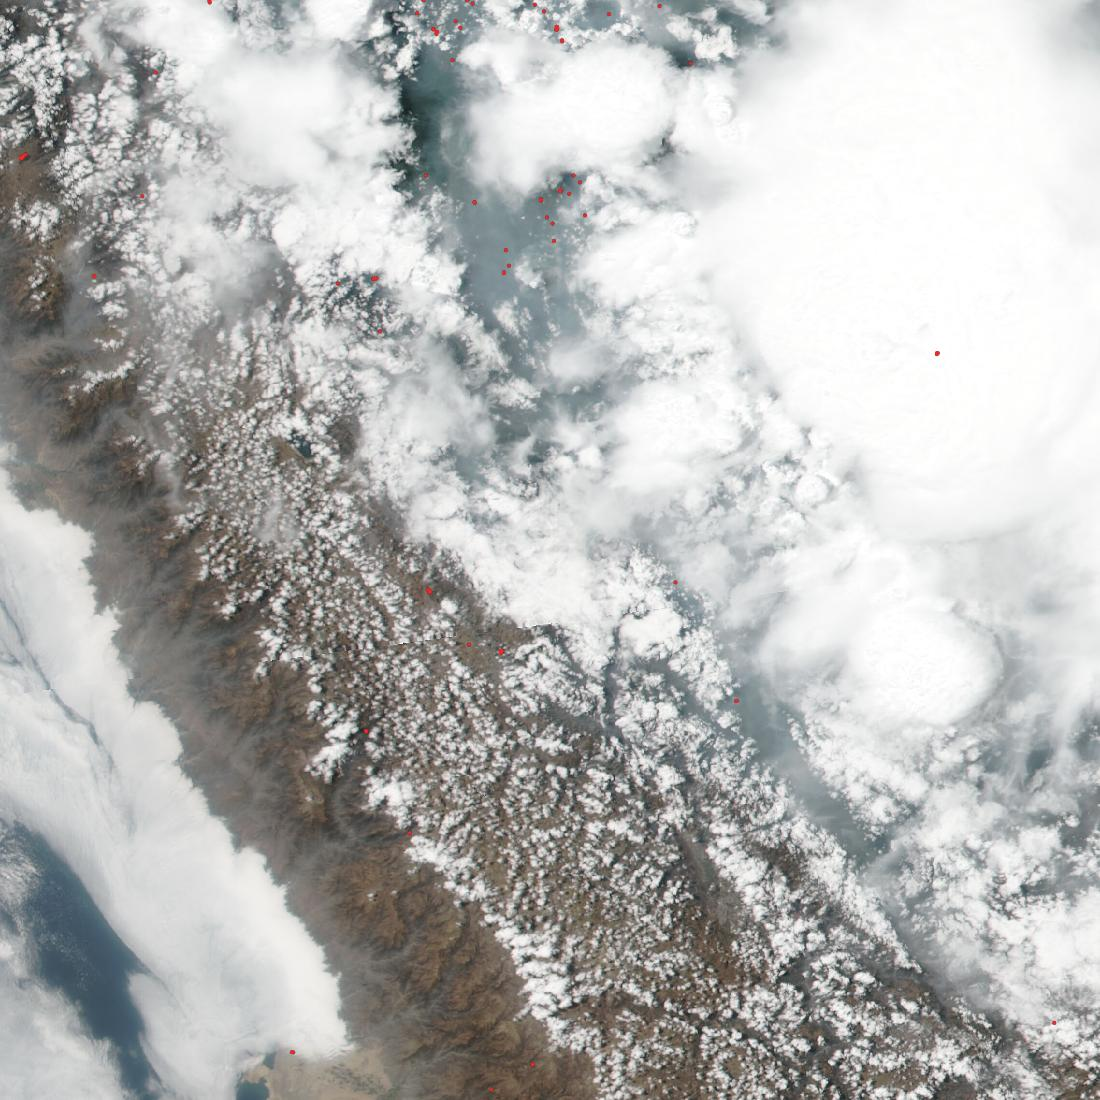
\includegraphics[width=\linewidth]{figuras/wv_viirs.jpg}};
    \begin{scope}[x={(img.south east)},y={(img.north west)}]
      \draw[white,thick] (0.458,0.386) circle (0.022);
      \node[white,fill=black,fill opacity=.75,text opacity=1,inner sep=2pt,font=\footnotesize\bfseries,anchor=west] at (0.49,0.386) {Huancayo};
    \end{scope}
  \end{tikzpicture}
  \caption{VIIRS en Suomi NPP: color verdadero y detecciones de 375~m.}
\end{subfigure}\hfill
\begin{subfigure}[t]{0.485\textwidth}
  \begin{tikzpicture}
    \node[inner sep=0,anchor=south west] (img) at (0,0) {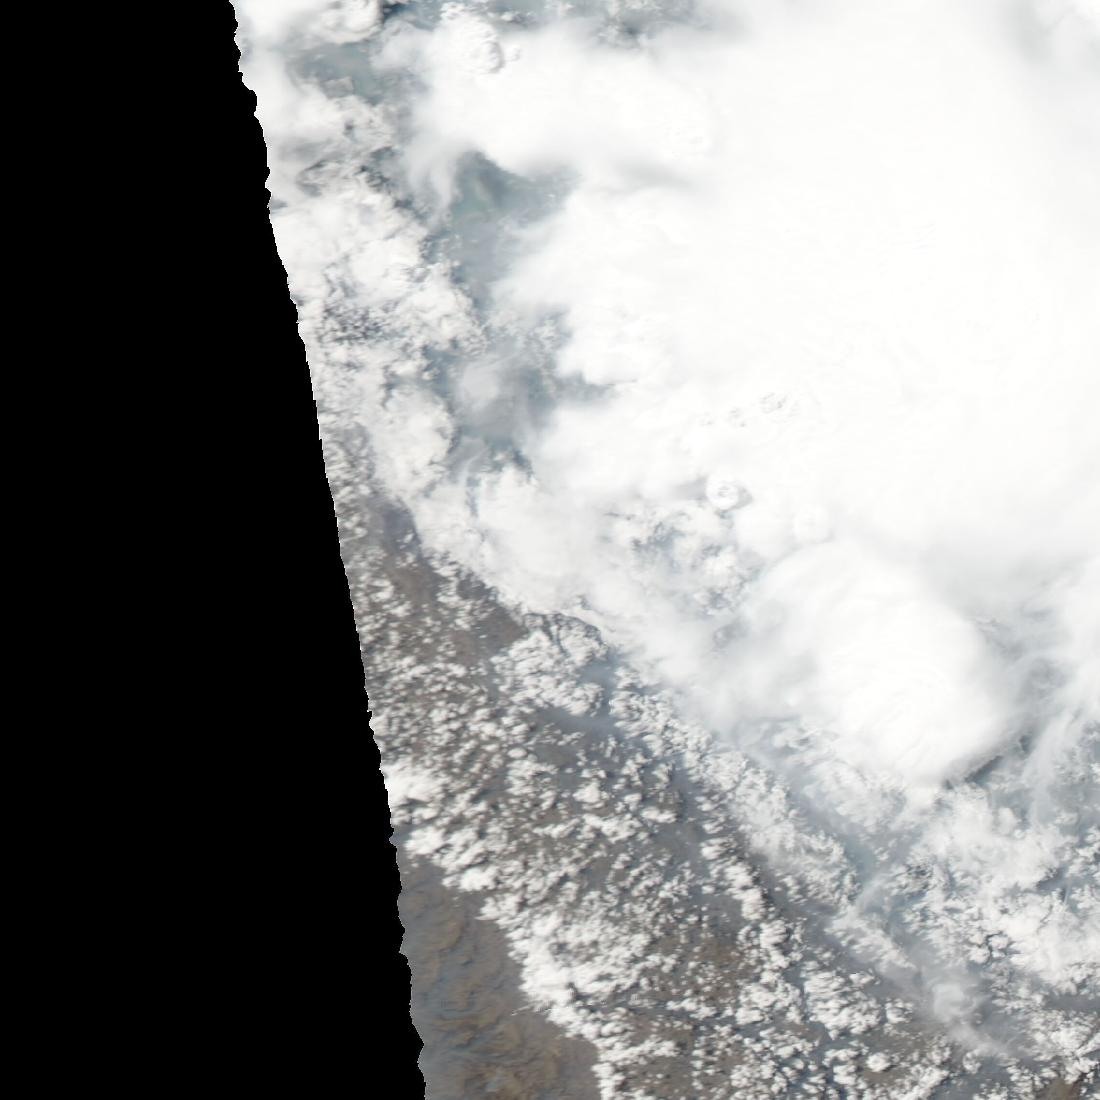
\includegraphics[width=\linewidth]{figuras/wv_modis.jpg}};
    \begin{scope}[x={(img.south east)},y={(img.north west)}]
      \draw[white,thick] (0.458,0.386) circle (0.022);
      \node[white,fill=black,fill opacity=.75,text opacity=1,inner sep=2pt,font=\footnotesize\bfseries,anchor=west] at (0.49,0.386) {Huancayo};
      \node[white,font=\footnotesize,align=center] at (0.17,0.62) {sin datos:\\ fuera de la\\ franja de Aqua};
    \end{scope}
  \end{tikzpicture}
  \caption{MODIS en Aqua: color verdadero y detecciones de 1~km.}
\end{subfigure}
\caption{El centro del Perú el 15 de septiembre de 2024 visto por los dos sensores de la tarde.
Imágenes de NASA Worldview (capas \emph{Corrected Reflectance} y \emph{Fires and Thermal
Anomalies}). El círculo marca la posición de Huancayo.}
\label{fig:worldview}
\end{figure}

Vale la pena mirarlas despacio, porque en un solo par de imágenes aparecen tres de los fenómenos
estudiados hasta aquí.

\textbf{El hueco de MODIS.} Toda la mitad izquierda de la imagen de Aqua está en negro. No es un
fallo: ese día, el borde de la franja de Aqua pasó por el centro del recuadro y la costa y buena
parte de la sierra quedaron en el hueco entre dos órbitas (sección~\ref{sec:huecos}). VIIRS, con
su franja más ancha, cubre el recuadro entero.

\textbf{Las detecciones.} En la imagen de VIIRS se cuentan varias decenas de puntos rojos,
agrupados sobre todo en la selva central, en la parte superior. En la imagen de Aqua no se
distingue ninguno. Parte de esos fuegos caía fuera de la franja de Aqua; los demás estaban en su
borde extremo, donde los píxeles de MODIS miden varios kilómetros
(capítulo~\ref{cap:escaneo}).

\textbf{Las nubes.} Más de la mitad de la escena está cubierta. Todo lo que ardiera bajo la gran
masa nubosa de la derecha es invisible para ambos sensores (capítulo~\ref{cap:atmosfera}). El
humo, en cambio, se aprecia como un velo grisáceo sobre la selva sin impedir las detecciones.

\begin{atencion}[Lo que esta imagen dice y lo que no]
Este es un solo día, elegido porque ilustra bien las diferencias. Otros días la franja de Aqua
cubre la zona de lleno y ambos sensores detectan fuegos. La imagen no demuestra que <<MODIS no
ve nada>>, sino por qué el conteo diario de MODIS en latitudes bajas es irregular y por qué
ninguna comparación entre los sensores debe apoyarse en días sueltos. La comparación válida es
la de muchos días acumulados.
\end{atencion}

\section{El final de MODIS}

Terra y Aqua llevan más de dos décadas en órbita. Sus horas de paso derivan al dejar
de mantenerse sus órbitas nominales; NASA indica que ese cambio debe evaluarse según
el uso científico. No fijamos aquí una fecha definitiva de cierre de ambas misiones:
el plan y el estado deben comprobarse en las fuentes oficiales.\fuente{transition}

La continuidad también afecta a VIIRS. NOAA anunció el fin de entrega de datos de
Suomi NPP el 2 de noviembre de 2026 a las 15:40 UTC.\fuente{noaa-snpp} Sus observaciones
históricas permiten calibrar, pero un sistema que continúe después necesita evaluar
el enlace con NOAA-20 o NOAA-21. Compartir familia instrumental no garantiza igualdad
de calibración, hora exacta ni cobertura. La comparación se repite en su propio solape.

\resumen

\begin{itemize}
  \item \textbf{MODIS} (Terra y Aqua) detecta fuego con píxeles de 1~km usando las bandas 21 y
  22 (3,96~\um) y 31 (11~\um). \textbf{VIIRS} (Suomi NPP, NOAA-20, NOAA-21) lo hace con píxeles
  de 375~m usando I4 (3,74~\um) e I5 (11,45~\um).
  \item Un detector se \textbf{satura} cuando la radiancia supera su máximo. MODIS usa dos
  bandas para cubrir fondo y fuego; la banda I4 de VIIRS se satura a 367~K.
  \item VIIRS cuenta más que MODIS por dos familias de motivos: \emph{ve fuegos que MODIS no ve}
  (píxel pequeño, bordes, huecos) y \emph{cuenta más veces lo mismo} (más píxeles por fuego, más
  satélites).
  \item La razón entre ambos conteos \textbf{no es constante}: depende del tipo de fuego, de la
  región y de la época.
  \item La continuidad exige evaluar tanto la transición MODIS--VIIRS como los cambios
  de plataforma dentro de VIIRS; Suomi NPP ya no aporta datos nuevos tras el cierre anunciado.
\end{itemize}

\ejercicios

\begin{enumerate}
  \item Calcula cuántos píxeles de VIIRS de 375~m caben en un píxel de MODIS, en el nadir y en
  el borde de la franja de MODIS (usa los tamaños de la tabla~\ref{tab:comparacion}).
  \item Para cada fila de la tabla~\ref{tab:comparacion}, indica si la diferencia pertenece a
  la familia <<ve fuegos que el otro no ve>> o a la familia <<cuenta más veces lo mismo>>, o a
  ninguna.
  \item ¿Por qué MODIS necesita dos bandas a 3,96~\um? ¿Qué pasaría si solo tuviera la 22? ¿Y si
  solo tuviera la 21?
  \item Una región tiene casi exclusivamente quemas de rastrojo de menos de una hectárea. Otra
  tiene incendios forestales de miles de hectáreas. ¿En cuál esperas una razón VIIRS/MODIS
  mayor? Justifica con las dos familias de diferencias.
  \item En la figura~\ref{fig:worldview}, ¿qué proporción aproximada del recuadro quedó sin
  observar por Aqua? Si eso ocurre uno de cada seis días, ¿qué fracción de las oportunidades
  diurnas de Aqua se pierde en esa zona por los huecos?
  \item Cuando MODIS se apague, ¿qué parte del ciclo diurno del fuego dejará de observarse? ¿Qué
  tipo de fuego crees que se verá más afectado?
\end{enumerate}

\lecturas

Los dos artículos fundamentales son Giglio, Schroeder y Justice (2016) para el algoritmo de
MODIS, y Schroeder, Oliva, Giglio y Csiszar (2014) para el de VIIRS de 375~m. Las referencias
completas y sus enlaces están en el apéndice~\ref{ap:fuentes}.
